\section {PlanesGraphicsScene}

\subsection{Main Window}

Similar to the PlanesWidget variant, the main window of the project is an object of a class derived from QMainWindow. In the constructor it creates the View - PlanesGSView - and the controller - PlaneRound - the game engine. 

\begin{figure}[h]
	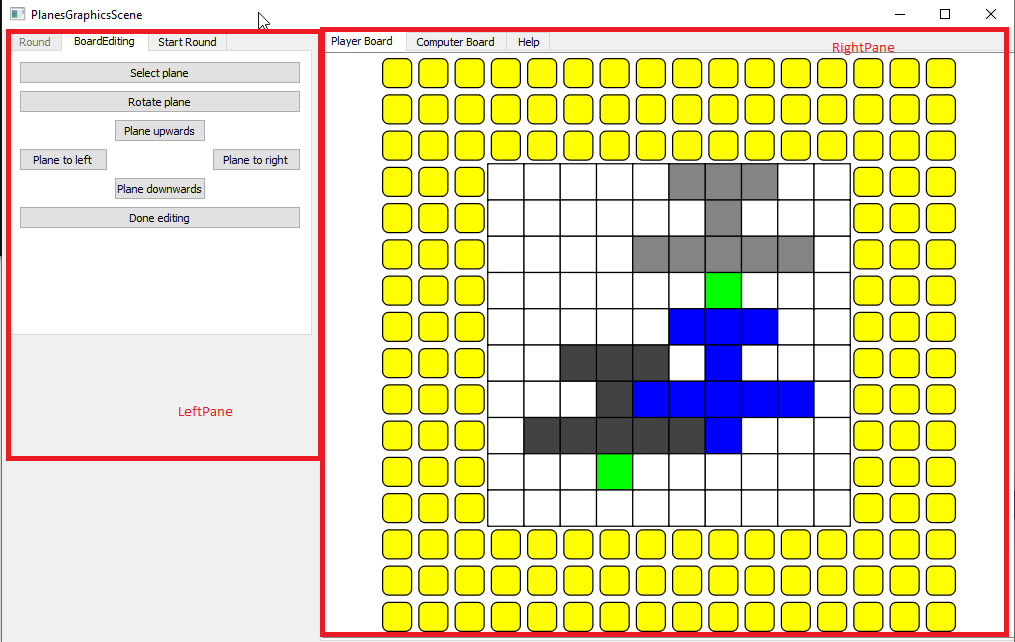
\includegraphics[width = \textwidth]{PlanesGraphicsScene_BoardEditing_WidgetNames.png}
	\caption{Simplified Layout of PlanesGraphicsScene}
	\label{fig:planesgraphicsscene_boardediting_widgetnames}
\end{figure}

The member variables for the PlanesGSView are:

\begin{lstlisting}

	//PlaneGrid objects manage the logic of a set of planes on a grid
	//as well as various operations: save, remove, search, etc.
	PlaneGrid* m_playerGrid;
	PlaneGrid* m_computerGrid;
	
	//PlaneRound is the object that coordinates the game
	PlaneRound* m_round;
	
	LeftPane* m_LeftPane;
	RightPane* m_RightPane;

\end{lstlisting}

Better as in the PlanesWidget project, the ComputerLogic object is not extracted from the PlaneRound anymore, only the two PlaneGrid objects are, which is still not satisfactory. The widgets composing the GUI are grouped under two principal widgets: LeftPane and RightPane.

The layout of the PlanesGSView is defined as follows:

\begin{lstlisting}
	CustomHorizLayout* hLayout = new CustomHorizLayout(this);
	m_LeftPane = new LeftPane(this);
	m_LeftPane->setMinWidth();
	//m_LeftPane->setSizePolicy(QSizePolicy::Fixed, QSizePolicy::Expanding);
	
	m_RightPane = new RightPane(*m_playerGrid, *m_computerGrid, this);
	m_RightPane->setMinWidth();
	
	hLayout->addWidget(m_LeftPane);
	hLayout->addWidget(m_RightPane);
	setLayout(hLayout);
\end{lstlisting} 

In principle it is a customized horizontal layout (see \ref{custom_qt_layout}) containing the LeftPane and RightPane widgets (see Figure \ref{fig:planesgraphicsscene_boardediting_widgetnames}). 

\subsection{LeftPane}
The LeftPane widget is a QTabWidget, a widget displaying more tabs. There is one tab for each game stage. To each of these tabs corresponds one widget: m\_BoardEditingWidget, m\_GameWidget, m\_StartGameWidget.

The class defines methods to interact when a new game stage starts:

\begin{lstlisting}
    void activateGameTab();
	void activateEditorTab();
	void activateStartGameTab();
\end{lstlisting}

It also defines signals that symbolize clicks on the different buttons in the interface:

\begin{lstlisting}
    void selectPlaneClicked(bool);
	void rotatePlaneClicked(bool);
	void upPlaneClicked(bool);
	void downPlaneClicked(bool);
	void leftPlaneClicked(bool);
	void rightPlaneClicked(bool);
	void doneClicked();
	void startNewGame();
\end{lstlisting}

Finally it defines how the widget reacts to external events, throught the following slots:

\begin{lstlisting}

	/**
	* @brief When planes overlap deactivate the done button
	* @param planesOverlap - received info from corresponding signal
	*/
	void activateDoneButton(bool planesOverlap);
	
	/**
	* @brief Activate the game tab when the done button is clicked
	*/
	void doneClickedSlot();
	
	/**
	* @brief activates the editing board tab and the buttons in it
	*/
	void activateEditingBoard();
	
	/**
	* @brief Updates the statistics in the left pane
	*/
	void updateGameStatistics(const GameStatistics& gs);
	
	/**
	* @brief
	* Hide the other tabs.
	*/
	void endRound(bool isPlayerWinner);

\end{lstlisting}

\subsection{RightPane}

The RightPane is a QTabWidget as well with 3 tabs: player's game board, computer's game board and the help page.

The RightPane emits two signals:

\begin{lstlisting}
	void planePositionNotValid(bool);
	void guessMade(const GuessPoint& gp);
\end{lstlisting}

and reacts to signals with the slots:

\begin{lstlisting}
    void resetGameBoard();
	void selectPlaneClicked(bool);
	void rotatePlaneClicked(bool);
	void upPlaneClicked(bool);
	void downPlaneClicked(bool);
	void leftPlaneClicked(bool);
	void rightPlaneClicked(bool);

	/**
	* @brief Switch to computer tab and start looking for planes.
	* Change the internal state of the player's and computer's boards to game stage
	*/
	void doneClicked();
	
	/**
	* @brief Display winner message in the player and computer boards.
	* Block mouse click events in the computer board.
	*/
	void endRound(bool isPlayerWinner);
	void startNewGame();
	void showComputerMove(const GuessPoint& gp);
\end{lstlisting}

The core of the RightPane class are the two game boards, implemented in the classes: PlayerBoard and ComputerBoard.

\subsection{The Game Boards}

Both PlayerBoard and ComputerBoard derive from the class GenericBoard, that provides the tools to interact with a PlaneGrid object from the game controller in order to display the planes and guesses throughout the game.

PlayerBoard and ComputerBoard in PlanesGraphicsScene correspond to GameRenderArea from the PlanesWidget. GenericBoard in PlanesGraphicsScene corresponds to BaseRenderArea in PlanesWidget.

The most important improvement brought by GenericBoard when compared to BaseRenderArea is that it is not a QWidget where the paintEvent() method was overriden, but it uses a specialized framework of Qt: the GraphicsScene/GraphicsView framework.

\subsection{Qt Concepts}

\subsubsection{Implementing a Custom Layout} \label{custom_qt_layout}

A custom layout was used for the PlanesGSView class:

\begin{lstlisting}
int CustomHorizLayout::count() const
{
	return m_ItemsList.size();
}

QLayoutItem* CustomHorizLayout::itemAt(int idx) const
{
	// QList::value() performs index checking, and returns 0 if we are
	// outside the valid range
	return m_ItemsList.value(idx);
}

QLayoutItem* CustomHorizLayout::takeAt(int idx)
{
	// QList::take does not do index checking
	return idx >= 0 && idx < m_ItemsList.size() ? m_ItemsList.takeAt(idx) : 0;
}

void CustomHorizLayout::addItem(QLayoutItem* item)
{
	if (count() < 2)
		m_ItemsList.append(item);
}

CustomHorizLayout::~CustomHorizLayout()
{
	QLayoutItem *item;
	while ((item = takeAt(0)))
	delete item;
}

void CustomHorizLayout::setGeometry(const QRect &r)
{
	QLayout::setGeometry(r);
	
	///only two widgets can lie in this layout
	if (count() != 2)
	return;
	
	QList<int> scalHoriz;
	
	scalHoriz.append(20);
	scalHoriz.append(80);
	
	int w = r.width() - (count() + 1) * spacing();
	int i = 0;
	int curX = 0;
	while (i < count()) {
		QLayoutItem *o = m_ItemsList.at(i);
		int wtemp = (w * scalHoriz[i]) / 100;
		int htemp = r.height();
		if (i == 0) {
			wtemp = std::max(wtemp, o->minimumSize().width());
			htemp = std::max(r.height() / 2, o->minimumSize().height());
		} else {
			wtemp = std::max(r.width() - curX - spacing(), o->minimumSize().width());
		}
		QRect geom(r.x() + curX + (i + 1) * spacing(), r.y(), wtemp, htemp);
		o->setGeometry(geom);
		++i;
		curX += wtemp;
	}
}

QSize CustomHorizLayout::sizeHint() const
{
	QSize s(0,0);
	int n = m_ItemsList.count();
	if (n > 0)
		s = QSize(1000, 600); //start with a nice default size
	int i = 0;
	while (i < n) {
		QLayoutItem *o = m_ItemsList.at(i);
		s = s.expandedTo(o->sizeHint());
		++i;
	}
	return s + n*QSize(spacing(), spacing());
}

QSize CustomHorizLayout::minimumSize() const
{
	QSize s(0,0);
	int n = m_ItemsList.count();
	int i = 0;
	while (i < n) {
		QLayoutItem *o = m_ItemsList.at(i);
		s = s.expandedTo(o->minimumSize());
		++i;
	}
	return s + n*QSize(spacing(), spacing());
}

\end{lstlisting}

The class CustomHorizLayout extends QLayout. It is a layout that accepts only two widgets, the condition is defined in the addItem() function. The most important function is setGeometry(). Here we define that given a total layout size w, the width of the LeftPane widget (the first to be added in the layout) is

\begin{lstlisting}
	std::max((w * 20) / 100;, o->minimumSize().width());
\end{lstlisting}

where o is the LeftPane widget, which has defined a minimumSize() based on the display size of strings that are to be displayed in the widget.

The RightPane should be displayed directly near the LeftPane with a width of 

\begin{lstlisting}
	std::max(r.width() - curX - spacing(), o->minimumSize().width());
\end{lstlisting}

That means it will take the remaining size width as long as this width is not smaller as the minimum width of the RightPane widget (which is defined in the minimumSize() function for the widget)

The other functions of the class are standard functions, like they are shown in tutorials on the Qt website.

\subsubsection {GraphicsScene - GraphicsView Framework of Qt}